\lesson{6}{18.10.2023}{Схема Бернулли, схема Уолкера, неравенство Крафта.}

\section{Схема Бернулли}

\begin{definition}
    Пусть $\delta_1,...,\delta_n$ — последовательность независимых одинаково распределенных
    случайных величин, каждая из которых принимает значение 1 с вероятностью $p$ и
    значение 0 с вероятностью $q = 1-p$. Такая вероятностная схема называется схемой Бернулли.

\end{definition}

\begin{definition}
    Случайная величина $\xi_n = \delta_1 + \ldots, \delta_n$ имеет биномиальное распределение:
    \[p(\xi_n = k) = C_{n}^{k} p^{k}q^{n-k}\]
\end{definition}

\begin{remark}
    Чтобы найти $\xi_n=k$ нужно чтобы $k$ из случайных величин $\delta_1,...,\delta_n$ принимали значение 1, остальные - 0. 
    Вероятность этого события при фиксированных местах единиц и нулей равна $p^kq^{n-k}$, и если учесть все возможные $C_n^k$ расположений этих мест, то получим $k-$ый член биномиального разложения $(p+q)^n$
\end{remark}

\begin{properties}
    Т.к. $E_{\xi_1} = p$ и $D_{\xi_1} = p - p^2 = pq$:

    \begin{enumerate}
        \item $E_{\xi} = np$
        \item $D_{\xi} = npq$
    \end{enumerate}

\end{properties}

\section{Случайные числа и схема Уолкера}

Дискретная случайная величина — это такая случайная величина,
значения которой могут быть не более чем счетными, то есть либо
конечными, либо счетными. Под счётностью имеется ввиду, что значения 
случайной величины можно занумеровать. 

В вычислительных машинах можно имитировать случайные эксперименты. 
В качестве источника случайности используются специальные программы - 
\textit{датчики случайных чисел}. Датчик при каждом обращении к нему вырабатывает 
некоторое число (обычно целое или вещественное число из фиксированного 
диапазона), и последовательность этих чисел по своему поведению очень 
похожа на последовательность независимых \textit{случайных величин, 
имеющих одинаковое равномерное распределение.}

Есть стандартные функции — генераторы (псевдо-)случайных чисел, 
которые выдают случайные натуральные числа в диапазоне $[0:n]$, либо 
вещественные из $[0:1)$. Равномерное распределение обладает таким
свойством, что вероятность того, что случайная величина принимает 
значения из некоторого множества, пропорциональна количеству 
элементов в нем. 
Или же что вероятность попадания в промежуток $[a,b] \subset$ $[0:1)$ 
равна длине этого промежутка.


\begin{definition}
    Равномерное (дискретное) распределение --- распределение на 
    конечном множестве, в котором все исходы равновероятны.
\end{definition}

\begin{eg}
    Равномерное распределение на множестве целых чисел от $k$ до $l:$ 
    $$p(\xi=S)=\frac{1}{l-k+1}, S \in [k:l]$$
\end{eg}

\begin{algoritm}[Схема Уолкера]
    Пусть мы умеем получать случайное число из диапазона $[0:1)$. 
    Требуется смоделировать вероятностную схему из $m$ исходов с заданными вероятностями $p_1, p_2, ..., p_m.$
    \begin{itemize}
        \item Назовём “донорами” те исходы, которые получили больше, чем им нужно, т.е. $p_i < \frac{1}{m}$.

        \item Назовём “реципиентами” те исходы, которые получили меньше, чем им нужно, т.е. $p_i > \frac{1}{m}$.
    \end{itemize}
    Алгоритм перераспределения:
    \begin{enumerate}
        \item Берём произвольного донора и реципиента.
        \item Донор отдаёт реципиенту излишек из своего отрезка.
        \item Отмечаем точку, где донор отдал излишек реципиенту -- барьер.
        \item После этого у донора остаётся ровно столько, сколько ему нужно, а реципиент мог как остаться реципиентом (ему дали слишком мало), так и перейти в доноры (дали с избытком).
    \end{enumerate}
    И так до тех пор, пока доноры и реципиенты не закончатся. 
    После проведения такой предварительной работы можно за $O(1)$ 
    генерировать случайные числа с нужным нам распределением следующим образом:
    \begin{enumerate}
        \item Генерируем случайное число $x$ из диапазона $[0:1)$.
        \item берем $\lfloor xm\rfloor$ -- номер интервала на отрезке.
        \item Сравниваем $x$ с барьером на этом отрезке: если $x$ больше, возвращаем реципиент, если меньше -- донора.
    \end{enumerate}
\end{algoritm}
$\newline$\\
Пример:\\    
$m = 5, p(A) = 0.24, p(B) = 0.03, p(C) = 0.28, p(D) = 0.11, p(E) = 0.34$

\begin{figure}[H]
    \centering
    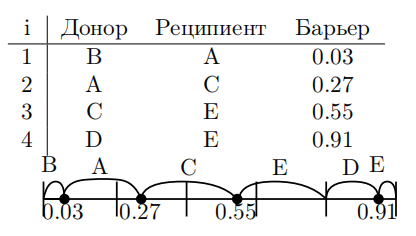
\includegraphics[width=0.5\textwidth]{alias.png}
    \label{fig:alias_method}
\end{figure}

\section{Двоичный поиск и неравенство Крафта.}

\begin{remark}
    Данная глава писалась с опорой на другие источники. Думаю, вы понимаете почему. $\bigodot \smile \bigodot $
\end{remark}

\begin{definition}
    Алфавит $A$ -- конечное непустое множество символов, $\alpha \in A^k$ -- строка длины $k$ над алфавитом $A$. 
\end{definition}

\begin{definition}
    $A^* = \bigcup_{k=0}^{\infty} A^k$ -- множество всех строк над алфавитом $A$ (слова). $\epsilon$ -- пустая строка.
\end{definition}

%про конкатенацию строк и ассоциативность и нейтральный элемент

\begin{definition}
    Кодом называется функция $\phi: A^* \rightarrow B^*$. $B$ -- алфавит кода.
\end{definition}

\begin{definition}
    Код называется декодируемым, если $\forall \alpha, \beta \in A^*: \alpha \neq \beta \implies \phi(\alpha) \neq \phi(\beta)$, т.е. $\phi$ -- инъекция.
\end{definition}

\begin{eg}
    Операция сжатия каким либо архиватором -- декодируемый код. $jpeg$ -- сжатие с потерей информации, недекодируемый код.
\end{eg}

\begin{definition}
    Разделяемый код -- код, в котором каждый символ алфавита $A$ кодируется отдельно, т.е. код -- функция $\phi: A \to B^*$.\\
    $\newline$\\
    Если хотим закодировать строку $\alpha = a_1a_2...a_n$, то $\phi(\alpha) = \phi(a_1)\phi(a_2)...\phi(a_n)$ (конкатенируем коды символов)
\end{definition}

\begin{definition}
    Префиксный код -- функция $\phi: A \to B^*$, такая, что 
    $\forall a, b \in A: \phi(a) \text{ -- не префикс } \phi(b)$, т.е.
     ни одно кодовое слово не является префиксом другого кодового слова.
\end{definition}

\begin{eg}
    Пример: $A = \{a, b, c\}, B = \{0, 1\}$\\
    $\phi(a) = 0, \phi(b) = 10, \phi(c) = 11 \implies \phi$ -- не префиксный код.
\end{eg}

\begin{theorem}
    Если код префиксный, то он однозначно декодируемый.
\end{theorem}

\begin{proof}
    Приведем алгоритм декодирования.

    Пусть дана $t = \phi(s)$, нужно найти $s$. Тогда будем из $t$ выделять 
    префикс (он будет один, т.к. код префиксный), который является кодом 
    некоторого символа $a_1$. Отрежем этот префикс от $t$. Так делаем, 
    пока $t$ не кончится. Получим $a_1a_2...a_n = s$.
\end{proof}

\begin{theorem}[неравенство Крафта]
    Для алфавита $A = \{c_1, ..., c_k\}$ можно построить однозначно декодируемый двоичный код с длинами кодовых слов $s_1, \ldots, s_k$ если:
    \[\sum_{i=1}^{k}2^{-s_i} \leq 1 \label{eq:Kraft} \eqno{2}\]
    
    И наоборот, если для чисел $s_1, \ldots, s_k$ выполняется неравенство $\ref{eq:Kraft}$, то существует однозначно декодируемый двоичный код в алфавите A.
\end{theorem}

\begin{proof}(Необходимость)
    %$\newline$
    %Не умоляя общности, будем считать, что 
    %$s_1 \leq s_2 \leq \ldots \leq s_k$. 
    %Тогда $2^{-s_1} \geq 2^{-s_2} \geq \ldots \geq 2^{-s_k}$\\
    %$\newline$\\
    %    Теперь распложим эти значения на отрезке $[0, 1]:$
    %
    %    \begin{tikzpicture}
    %        
    %        \draw[-, thick] (0,0) -- (5.4,0);
    %        
    %        
    %        \foreach \x in {1,2} {
    %            \draw (\x-1,0.1) -- (\x-1,-0.1);
    %            
    %            %\draw[dashed] (\x-1,0) -- (\x-1,0.5);
    %            \node[above] at (\x-0.5, 0.5) {$2^{-s_{\x}}$};
    %            \draw (\x-1,0) to[bend left=30] (\x,0);
    %        }
    %        \draw (2,0.1) -- (2,-0.1);
    %        \node[above] at (2.5, 0.5) {$2^{-s_{i}}$};
    %        \draw (2,0) to[bend left=30] (3,0);
    %        \draw (3,0.1) -- (3,-0.1);
    %        \node[above] at (3.5, 0.5) {$\ldots$};
    %        \draw (4,0.1) -- (4,-0.1);
    %        \node[above] at (4.5, 0.5) {$2^{-s_{k}}$};
    %        \draw (5,0.1) -- (5,-0.1);
    %        \draw (4,0) to[bend left=30] (5,0);
    %    
    %        
    %        
    %        \fill[black] (0,0) circle (0.05) node[below] {0};
    %        \fill[black] (5.4,0) circle (0.05) node[below] {1};
    %    \end{tikzpicture}
    Рассмотрим бинарное дерево T. Каждой вершине $r$ сопоставим число 
    $a_r = 2^{-l}$, где $l$ длина пути от корня до вершины $r$. Для 
    корня имеем $a_{root} = 1$.\\
    Заметим, что для любого узла, который не лист, справедливо неравенство:
    \[2^{-l} \geq \underbrace{2^{-(l+1)}}_{left} + \underbrace{2^{-(l+1)}}_{right}\]
    
    Просуммируем все узлы, которые не являются листьями и все узлы не корни, тогда справедливо неравенство:

    \[\sum_{nodes \setminus leaves} a_r \geq \sum_{nodes \setminus \{a_{root}\}} a_r\]

    После сокращения общих слагаемых в левой и правой частях неравенства получаем корень слева и все листья справа:

    \[a_{root} = 1 \geq \sum_{leaves} a_r = \sum_{i=1}^{k} 2^{-s_i}\]

\end{proof}

